% flashcards-title: Centimetre ruler and measured strip
% flashcards-desc: A ruler runs from zero to four centimetres with ten equal subdivisions per centimetre. A blue outlined strip begins at zero and ends at mark X at 3.4 centimetres, indicated by a dashed guide.
\documentclass[border=6pt]{standalone}
\def\pgfsysdriver{pgfsys-dvisvgm.def}
\usepackage{tikz}
\usetikzlibrary{arrows.meta,positioning,shapes.geometric}
\definecolor{mechInk}{HTML}{172033}
\definecolor{mechBlue}{HTML}{155EEF}
\definecolor{mechOrange}{HTML}{B54708}
\definecolor{mechPale}{HTML}{E8F0FF}
\definecolor{mechGray}{HTML}{667085}
\definecolor{mechLight}{HTML}{D0D5DD}
\tikzset{
  every picture/.style={font=\sffamily\large, text=mechInk},
  mech box/.style={draw=mechInk, line width=1.2pt, rounded corners=4pt,
    fill=white, align=center, minimum height=14mm, inner xsep=5mm},
  mech primary/.style={draw=mechBlue, line width=2.2pt},
  mech secondary/.style={draw=mechOrange, line width=2.2pt, dashed},
  mech guide/.style={draw=mechGray, line width=0.9pt, dashed},
  mech arrow/.style={-{Stealth[length=3.2mm,width=2.4mm]},
    draw=mechInk, line width=1.4pt, line cap=butt},
  mech axis/.style={draw=mechInk, line width=1.2pt},
  mech tick/.style={draw=mechInk, line width=1pt}
}

\begin{document}
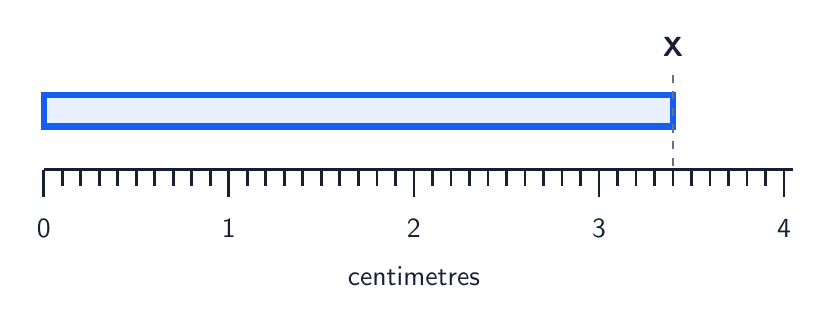
\begin{tikzpicture}[x=2.35cm,y=1cm]
  \fill[mechPale] (0,0.55) rectangle (3.4,0.95);
  \draw[mech primary] (0,0.55) rectangle (3.4,0.95);
  \draw[mech axis] (0,0) -- (4.05,0);
  \foreach \i in {0,...,40}{
    \pgfmathsetmacro{\xx}{\i/10}
    \ifnum\i=0
      \def\tickh{0.34}
    \else
      \pgfmathtruncatemacro{\rem}{mod(\i,10)}
      \ifnum\rem=0 \def\tickh{0.34}
      \else \def\tickh{0.20}\fi
    \fi
    \draw[mech tick] (\xx,0) -- (\xx,-\tickh);
  }
  \foreach \x in {0,...,4}{
    \node[below=5mm, font=\sffamily\normalsize] at (\x,0) {\x};
  }
  \node[below=11mm, font=\sffamily\normalsize] at (2,0) {centimetres};
  \draw[mech guide] (3.4,0.05) -- (3.4,1.22);
  \node[above=1mm, font=\sffamily\bfseries] at (3.4,1.22) {X};
\end{tikzpicture}
\end{document}
